\documentclass[compress,aspectratio=149,brazil]{beamer}
\mode<presentation>
\usepackage[portuguese]{babel}
\usepackage[T1]{fontenc}
\usepackage[utf8]{inputenc}
\usepackage{graphicx}
\usepackage{amsfonts}
\usepackage{amsmath}
\usepackage{booktabs}
\usepackage[table]{xcolor}

\title{Previsão de séries temporais por meio de aprendizado de máquina}
\author{Guilherme Chichanoski \\ \footnotesize \ttfamily{ra82174@uem.br}}
\institute{Orientadora: Profa. Dra. Valéria Delisandra Feltrim \\ \vspace{0.5cm} Universidade Estadual de Maringá \\ Departamento de Informática \\ Bacharelado em Ciência da Computação}
\date{\today}
\setbeamertemplate{footline}[frame number]

\begin{document}

\begin{frame}
    \titlepage{}
\end{frame}

\section{Introdução}

\begin{frame}{Introdução}
    \begin{itemize}
        \item Uma \textbf{Série temporal} é formada por um conjunto de
            observações realizadas ao longo do tempo;
        \item Essas observações são caracterizadas como estocásticas, ou seja,
            a observação atual pode ser dado segundo a observação anterior;
            \[ X_t = X_{t-1} + \epsilon \]
        \item A série pode ser obtida de diferentes fontes. Podendo, por
            exemplo, ser uma série financeira no caso de valores de ações;
        \item Este trabalho tem por objetivo estudar modelos de previsões para
            estas séries.
    \end{itemize}
\end{frame}

\begin{frame}{Introdução}
    \begin{example}[Exemplo de série temporal]
        \begin{figure}
            \centering
            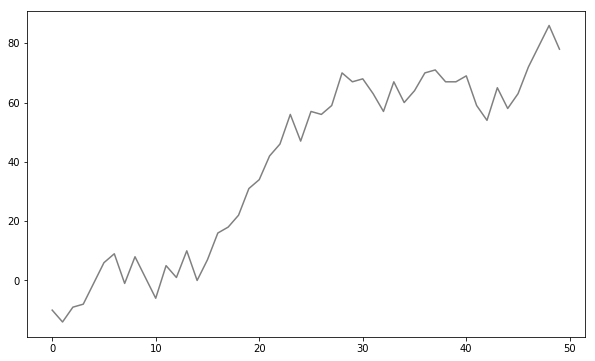
\includegraphics[scale=0.517]{../images/serie_exemplo.png}
            \\Fonte: Série gerada pelo autor para exemplo\label{fig:exemplo}
        \end{figure}
    \end{example}
\end{frame}

\begin{frame}{Introdução}
    \begin{itemize}
        \item Por que é interessante prever séries temporais?
        \begin{itemize}
            \item \textbf{Compreensão de comportamento:} Identificar padrões;
            \item \textbf{Aplicações:}
                \begin{itemize}
                    \item Financeira
                    \item Ambiental
                    \item Governamental
                \end{itemize}
            \item \textbf{Apoio a tomada de decisão:} Com uma previsão
                confiável o futuro se torna menos incerto, facilitando a tomada
                de decisão
        \end{itemize}
    \end{itemize}
\end{frame}

\begin{frame}{Introdução}
    \begin{itemize}
        \item<1-> A \textbf{previsão de séries temporais} tem uma abordagem
            estatística consolidada;
        \item<1-> A maioria da literatura existente emprega métodos
            \textbf{probabilísticos} descritos como métodos de Box:
        \begin{itemize}
            \item<2-> (Processos Auto Regressivos)AR;
            \item<3-> (Processos de Médias móveis)MA;
            \item<3-> AR+MA;
        \end{itemize}
    \item<4-> Abordagens utilizando \textbf{aprendizado de máquina} também são
            utilizadas, no entanto, com menor frequência
    \end{itemize}
\end{frame}

\begin{frame}{Objetivo}
    O objetivo deste  trabalho foi a implementação  de modelos probabilísticos,
    \textbf{ARIMA}, e de aprendizado de máquina, \textbf{MLP}. Identificar as
    diferenças e capacidades de cada modelo:

    \begin{enumerate}
        \item<2-> Produzir o modelo ARIMA considerando todas as etapas de definição
            do modelo;
        \item<3-> Obter o modelo de redes neurais artificiais;
        \item<4-> Comparar os modelos;
    \end{enumerate}
\end{frame}

\begin{frame}{Previsão}
    \begin{itemize}
        \item Etapas da previsão:
        \begin{enumerate}
            \item Definição do problema;
            \item Coleta dos dados;
            \item Análise dos dados;
            \item \alert<2>{Seleção e verificação do modelo}
            \item Avaliação do modelo;
            \item Publicação do modelo; e
            \item Monitoramento do desempenho do modelo.
        \end{enumerate}
    \end{itemize}
    \uncover<2->{\begin{alertblock}{Avaliação}
        Se o  modelo não  for adequado  durante a  etapa de  avaliação, deve-se
        retornar a  etapa anterior e  selecionar outro  modelo.
    \end{alertblock}}
\end{frame}

\begin{frame}{Série temporal}
    \begin{block}{Definição}
        \[\{X(t): t \in T\}\]
    \end{block}
    \begin{description}
        \item<2->[Contínua]
            \[T \subseteq \mathbb{R}\]
        \item<2->[\alert<3>{Discreta}]
            \[T \subseteq \{1,2,3,\ldots\}\]
    \end{description}
\end{frame}

\begin{frame}{Série estacionária}
    \begin{block}{Definição}
        Um Processo que se desenvolve em torno de uma média.
        \begin{description}
            \item[Estritamente estacionaria]
                A distribuição de probabilidade conjunto de \[X(t_1), \ldots, X(t_k)\] é igual a de \[X(t_1+\tau), \ldots, X(t_k+\tau)\]
            \item[\alert<2>{Fracamente estacionaria}]
                A função média deve ser constante.
        \end{description}
    \end{block}
\end{frame}

\begin{frame}{Sazonalidade e Tendencia}
    \begin{block}{Sazonalidade}
        Caracteriza a repetição ciclica de um comportamento e uma distância
        $s$ entre observações
    \end{block}
    \begin{block}{Tendencia}
        Comportamento da série observado durante um longo periodo de tempo.
        Podendo denotar crescimento ou decaimento da série.
    \end{block}
\end{frame}

\begin{frame}{Sazonalidade e Tendência}
    \begin{block}{Concentração de CO2}
        \begin{columns}
            \begin{column}{.7\textwidth}
                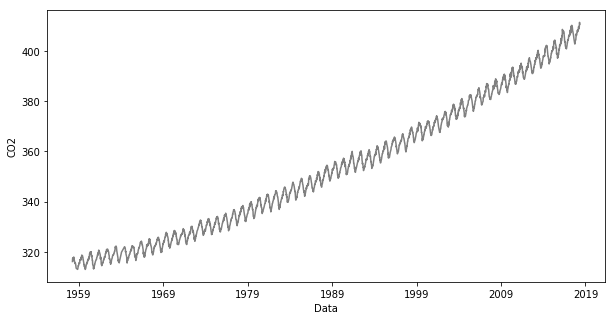
\includegraphics[width=\textwidth]{../images/co2.png}
            \end{column}
            \begin{column}{.3\textwidth}
                \begin{itemize}
                    \item Sazonalidade
                    \item Tendência
                \end{itemize}
            \end{column}
        \end{columns}
    \end{block}
\end{frame}

\begin{frame}{Filtros}
    \begin{block}{Médias Móveis}
        \begin{itemize}
            \item Remover sazonalidade
            \item Remover ruídos
        \end{itemize}
        \[ y_t = \sum_{j = -q}^{s}{a_{j}x_{t+j}} \]
        \only<2->{\alert{\[y_t = \frac{1}{2q + 1}\sum_{j=-q}^{q}{x_{t+j}}\]}}
    \end{block}
\end{frame}

\begin{frame}{Filtros}
    \begin{block}{Diferenciação}
        \begin{itemize}
            \item Remover tendência
            \item Tornar a série estacionária
        \end{itemize}
        \[
            y_t = x_t - x_{t-1}
        \]
    \end{block}
\end{frame}

\begin{frame}{Filtros}
    \begin{columns}
        \begin{column}{.5\textwidth}
            \begin{block}{Médias Móveis}
                \begin{itemize}
                    \item $q = 52$
                \end{itemize}
                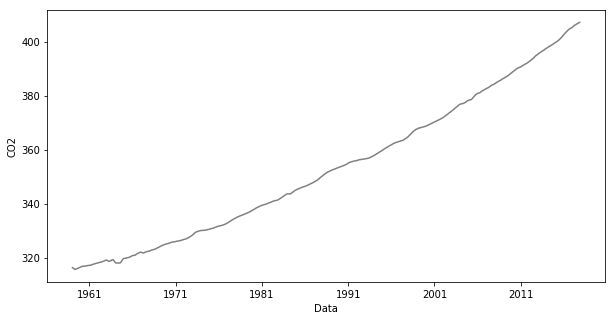
\includegraphics[width=\textwidth]{../images/co2_filtered.png}
            \end{block}
        \end{column}
        \begin{column}{.5\textwidth}
            \begin{block}{Diferenciação}
                \begin{itemize}
                    \item Uma diferenciação
                \end{itemize}
                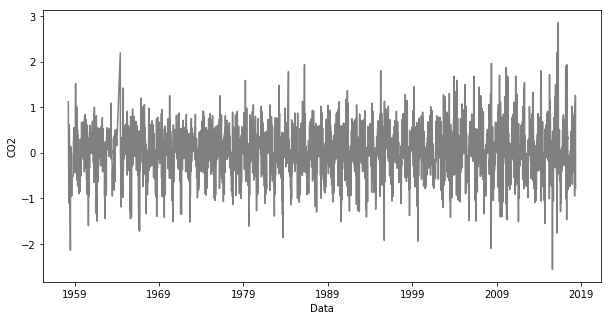
\includegraphics[width=\textwidth]{../images/co2_diff.png}
            \end{block}
        \end{column}
    \end{columns}
\end{frame}

\section{Modelos Probabilísticos}

\begin{frame}{Modelos Probabilísticos}
    \begin{itemize}
        \item Estocastico
        \item Método Box --- ARIMA
        \begin{itemize}
            \item $(p,d,q)$
            \item AR
            \item Integração
            \item MA
        \end{itemize}
    \end{itemize}
\end{frame}

\begin{frame}{Função de autocorrelação}
    \begin{itemize}
        \item Mede a correlação da série em função de si mesma deslocada em $k$
            lags
    \end{itemize}
    \[
    r_k = \frac{\sum_{t=1}^{n-k}{(x_t - \overline{x})(x_{t+k} -
    \overline{x})}}{\sum_{t=1}^{n}{(x_t - \overline{x})^2}}
    \]
    \begin{description}
        \item[Intervalo de confiança] \[\pm{}2/\sqrt{n}\]
    \end{description}
\end{frame}

\begin{frame}{Função de autocorrelação}
    \begin{block}{Exemplo --- CO2}
        \begin{center}
            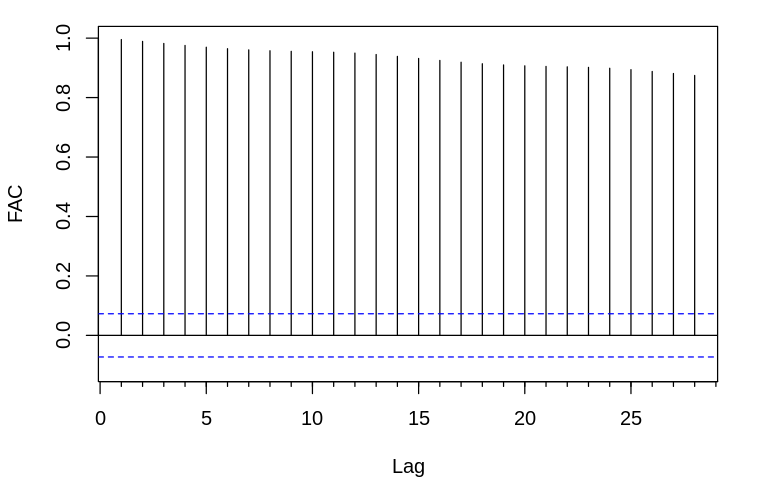
\includegraphics[width=.8\textwidth]{../images/acf_co2.png}
        \end{center}
    \end{block}
\end{frame}

\begin{frame}{Função de autocorrelação}
    \begin{block}{Exemplo --- CO2 (Diferenciado uma vez)}
        \begin{center}
            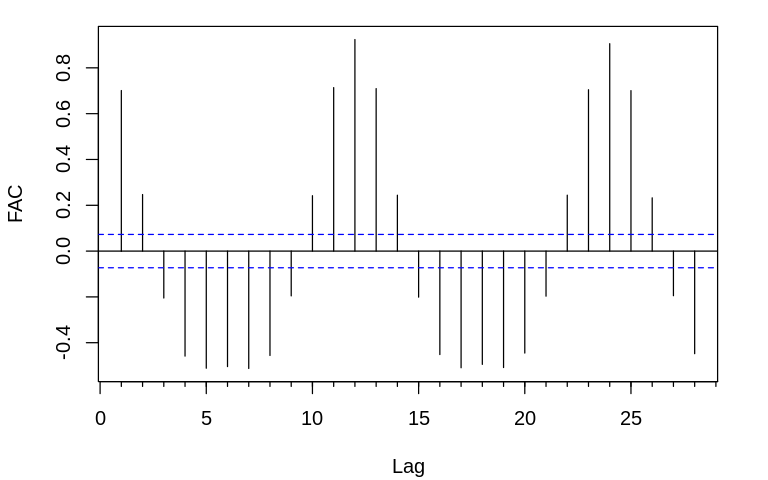
\includegraphics[width=.8\textwidth]{../images/acf_co2_diff.png}
        \end{center}
    \end{block}
\end{frame}

\begin{frame}{Função de autocorrelação parcial}
    \begin{itemize}
        \item Relevante na seleção da ordem do processo auto-regressivo
    \end{itemize}

    \[
    \phi_{kk} = \frac{r_k-\sum_{j=1}^{k-1}{\phi_{k-1,j}r_{k-j}}}{1-\sum_{j=1}^{k-1}{\phi_{k-1,j}r_{j}}}
    \]
\end{frame}

\begin{frame}{ARMA}
    \begin{description}
        \item[Auto-Regressivo (AR)]
            \[
                X_t = \sum_{i = 1}^{p}{\alpha_{i}X_{t-i}} + \epsilon_t
            \]
        \item[Médias Móveis (MA)]
            \[
                X_t = \epsilon_t - \theta_1\epsilon_{t-1} - \theta_2\epsilon_{t-2} - \cdots - \theta_{q}\epsilon_{t-q}
            \]
    \end{description}
    \begin{block}<2->{Modelo misto}
        \[
            X_t = \sum_{i = 1}^{p}{\alpha X_{t-i}} + \epsilon_t - \sum_{j = 1}^{p}{\theta \epsilon_{t-i}}
        \]
    \end{block}
\end{frame}

\begin{frame}{ARIMA}
    Nos casos que a série não for estacionaria é necessaria realização de pelo
    menos uma diferenciação. Este procedimento no modelo ARIMA é denotado pelo
    I, ou seja, a integração.

    \begin{block}{Modelo}
        \[
            (1 - \alpha_1B-\cdots-\alpha_pB^p)(1-B)^dy_t=(1+\theta_1B+\cdots+\theta_qB^q)\epsilon_t
        \]
    \end{block}
\end{frame}

\begin{frame}{Seleção do modelo}
    Segundo o metodo de Box devemos analisar a \textbf{FAC} e a \textbf{FACP}
    para determinar o modelo que mais se aproximado do adequado.

    \begin{table}[ht]
        \centering
        \begin{tabular}{l l l}
            \multicolumn{1}{c}{Modelo} & \multicolumn{1}{c}{FAC} & \multicolumn{1}{c}{FACP} \\
            \toprule
            Série aleatória  & 0                           & 0                        \\
            AR (p)           & decaimento exponencial      & 0 após $p$ \textit{lags} \\
            MA (q)           & 0 após $q$ \textit{lags}    & decaimento exponencial   \\
        \end{tabular}
    \end{table}
\end{frame}

\begin{frame}{Seleção do modelo}
    \begin{itemize}
        \item Modelo deve ser avaliado utilizando o \textbf{FAC}
        \item<2-> Parcimonioso
    \end{itemize}
    \begin{block}<2->{AIC}
        \[
            AIC = -2\log{L}+2(p+q+1)
        \]
    \end{block}
\end{frame}

\begin{frame}{Determinação dos coeficientes}
    \begin{description}
        \item[\alert<2>{Maximação da função \textit{likelihood}}]
        \[
            L(\theta) = \prod_{i=1}^{n}{q(x_i;\theta)}
        \]
        \item[Equaçã̀o de Yule Walker]
        \[
            \begin{pmatrix}
                r_1\\
                r_2\\
                \vdots\\
                r_{p-1}\\
                r_p
            \end{pmatrix} =
            \begin{pmatrix}
                1 & r_1 & r_3 & \cdots & r_{p-2} & r_{p-1} \\
                r_1 & 1 & r_1 & \cdots & r_{p-3} & r_{p-2} \\
                & & \vdots & & \vdots & \\
                r_{p-2} & r_{p-3} & r_{p-4} & \cdots & 1 & r_1 \\
                r_{p-1} & r_{p-2} & r_{p-3} & \cdots & r_1 & 1 \\
            \end{pmatrix}
            \begin{pmatrix}
                \alpha_1\\
                \alpha_2\\
                \vdots\\
                \alpha_{p-1}\\
                \alpha_p
            \end{pmatrix}
        \]
    \end{description}
\end{frame}

\subsection{Aprendizado de Máquina}

\begin{frame}{Aprendizado de máquina}
    \begin{block}{Definição}
        Identificação de padrões a partir dos dados
    \end{block}
    \begin{description}
        \item[Classificação]
        \item[\alert<2>{Regressão}]
        \item[Aprendizado não supervisionado]
        \item[Aprendizado por reforço]
    \end{description}
\end{frame}

\begin{frame}{Perceptron}
    \begin{itemize}
        \item Inspirados em neurônios
    \end{itemize}
    \begin{columns}
        \begin{column}{.5\textwidth}
            \[
                v(x) = \sum_{i=1}^{m}{w_i  x_i + b}
            \]
        \end{column}
        \begin{column}{.5\textwidth}
            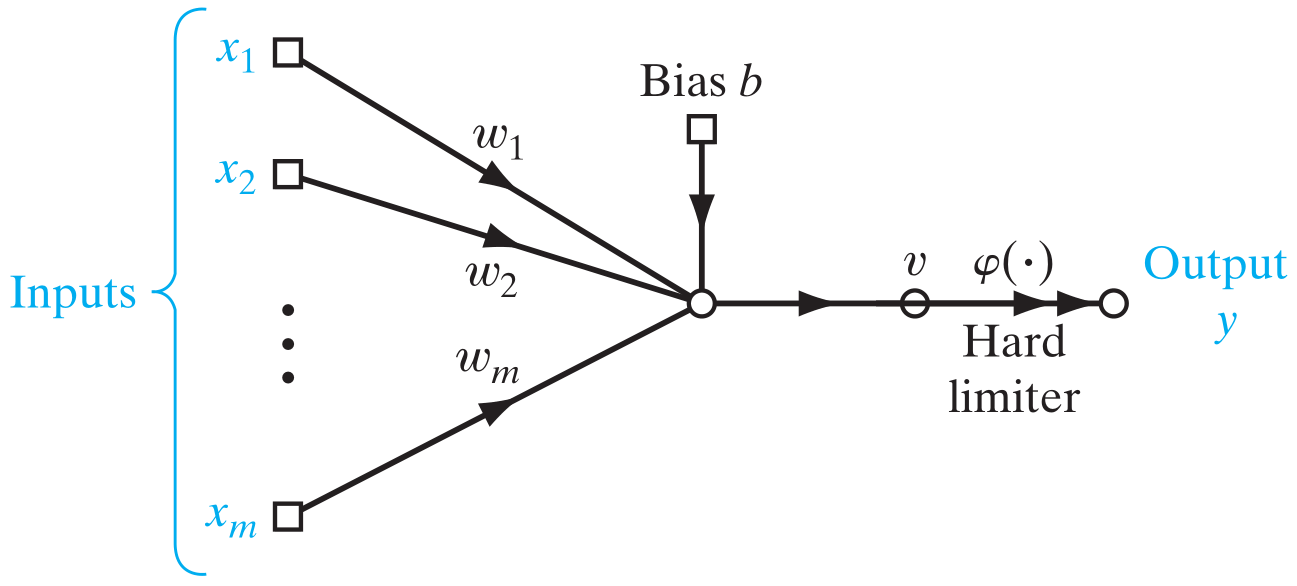
\includegraphics[width=\textwidth]{../images/perceptron.png}
        \end{column}
    \end{columns}
\end{frame}

\begin{frame}{Redes neurais de múltiplas camadas}
    \begin{columns}
        \begin{column}{.4\textwidth}
            \begin{enumerate}
                \item Camada de entrada
                \item Camadas escondidas
                \item Camada de saída
            \end{enumerate}
        \end{column}
        \begin{column}{.6\textwidth}
            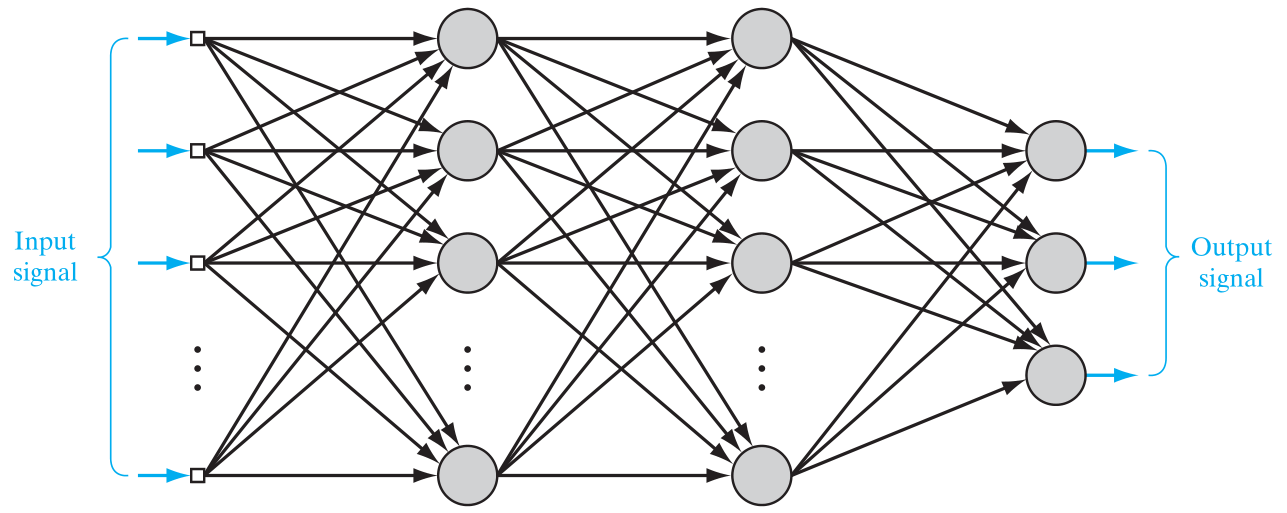
\includegraphics[width=\textwidth]{../images/neuralNetwork.png}
        \end{column}
    \end{columns}
\end{frame}

\begin{frame}{Função de perda (loss)}
    Durante o treinamento a função para avaliação e calculo do aprendizado é a
    seguinte:
    \[
        MSE = \frac{1}{n}\sum_{i=1}^{n}{{(Y_i - \hat{Y}_i)}^2}
    \]
\end{frame}

\begin{frame}{Aprendizado}
    O aprendizado ocorre utilizando o método de retropropagação, calculando os
    novos pesos do perceptron partindo da avaliação do resultado obtido com os
    valores reais.

    Os novos pesos serão dados pela seguinte equação:
    \[
        w_{n+1} = w_n - \alpha \frac{\partial L(x,w_t)}{\partial w_t}
    \]
\end{frame}

\section{Desenvolvimento}

\begin{frame}{Ferramentas utilizadas}
    \begin{description}
        \item[python]
            \begin{itemize}
                \item statsmodels
                \item pandas
                \item tensorflow
                \item scikit-learn
            \end{itemize}\\
        \item[R]
            \begin{itemize}
                \item forecast
                \item ggplot
                \item tseries
            \end{itemize}
    \end{description}
\end{frame}

\begin{frame}{Base de dados}
    S\&P500 --- Indice dos valores das 500 maiores empresas negociadas
    publicamente.
    \begin{center}
        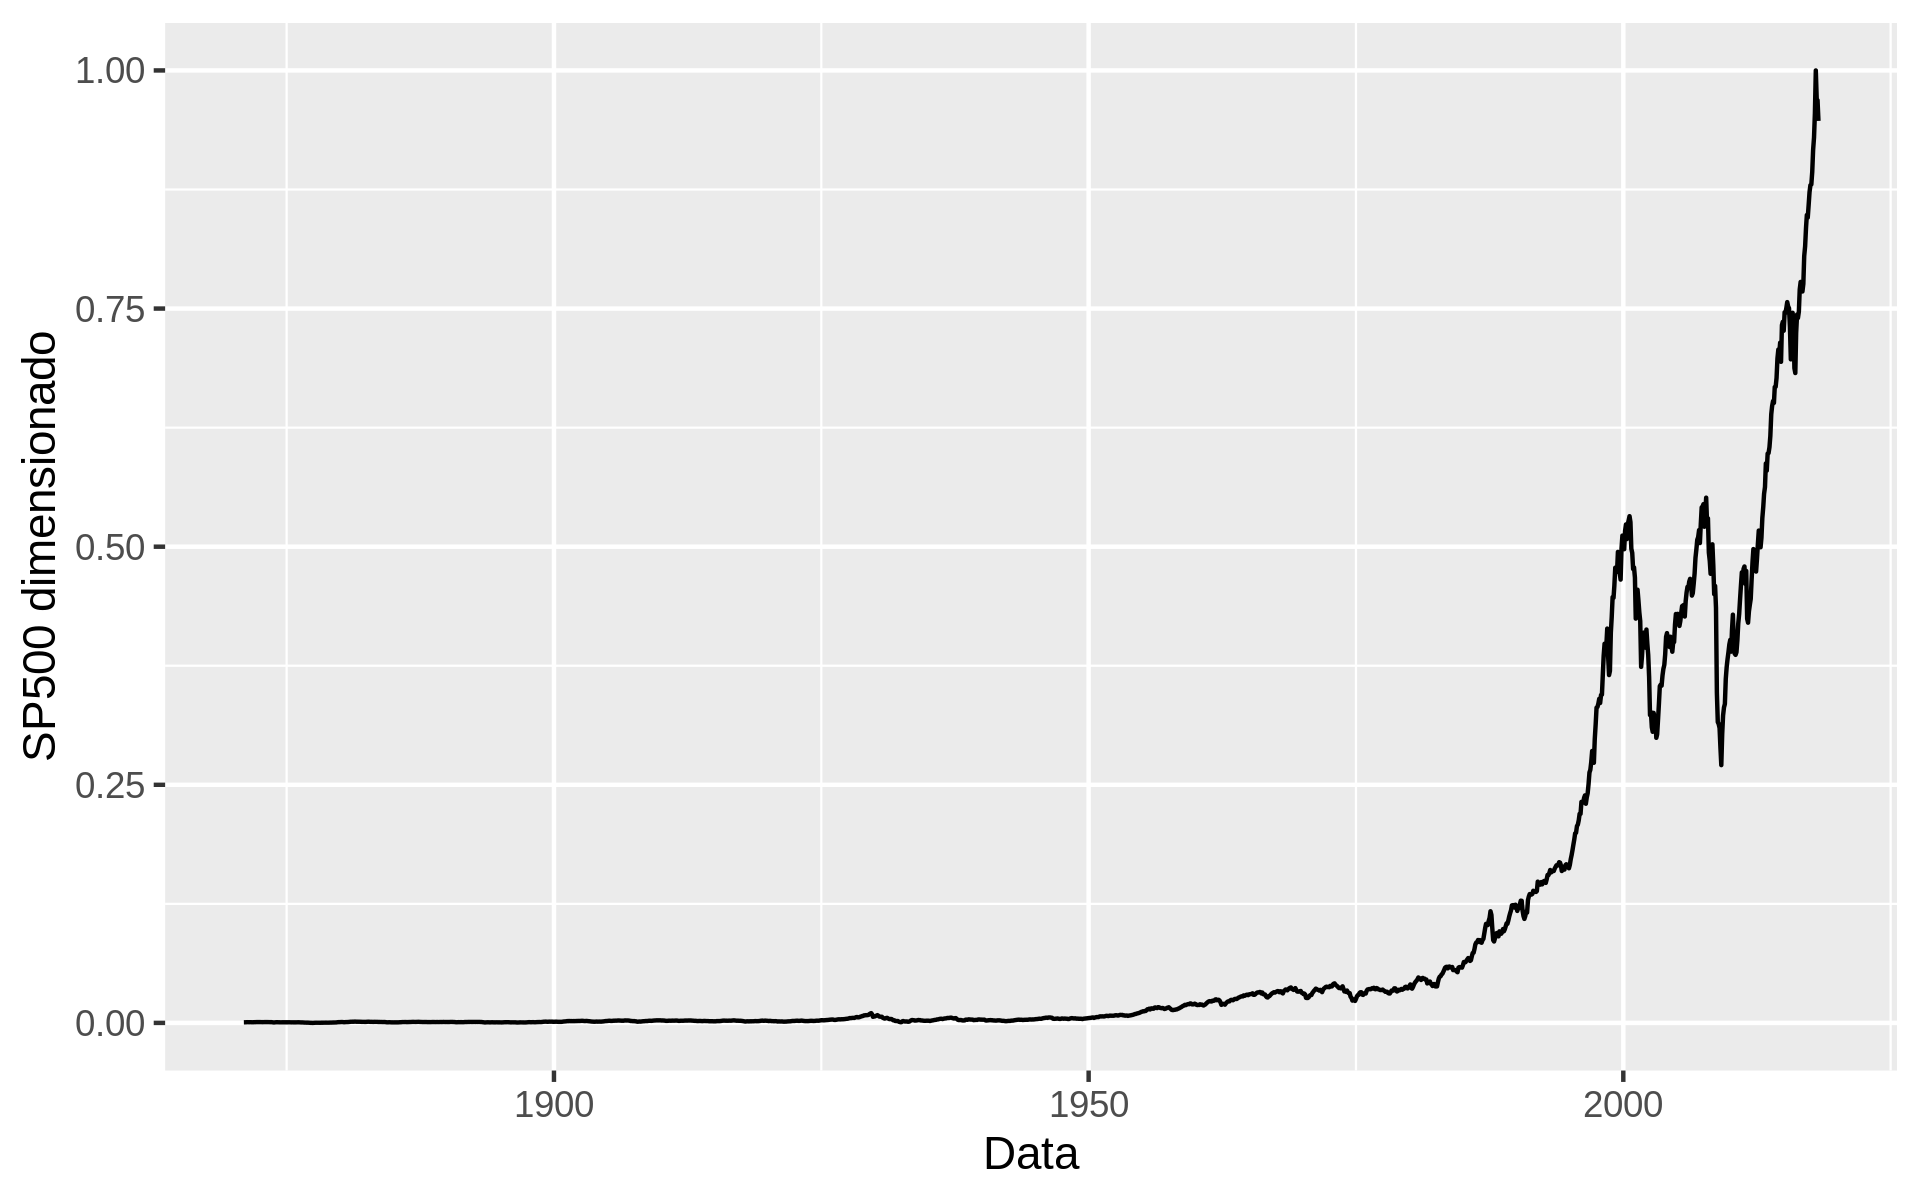
\includegraphics[width=.8\textwidth]{../images/SP500.png}
    \end{center}
\end{frame}

\begin{frame}{Preparação dos dados}
    Não foi identificado \textit{outliers} ou dados que necessitassem remoção.

    \begin{description}
        \item[Normalização]
            \[
                \begin{split}\label{eq:minmaxscaler}
                    &x_{std} = \frac{x - \min x}{\max x-\min x}\\
                    &x_{scaled} = x_{std} * (max-min)+min
                \end{split}
            \]
        \item[Divisão Treino/Teste]
            70\% Treino / 30\% Teste
    \end{description}

    \uncover<2>{\alert{Todos as análises foram feitas utilizando o conjunto de
        treino e as validações utilizando o conjunto de teste}}
\end{frame}

\begin{frame}{Análise da série}
    \begin{block}{Função de autocorrelação}
        \begin{center}
            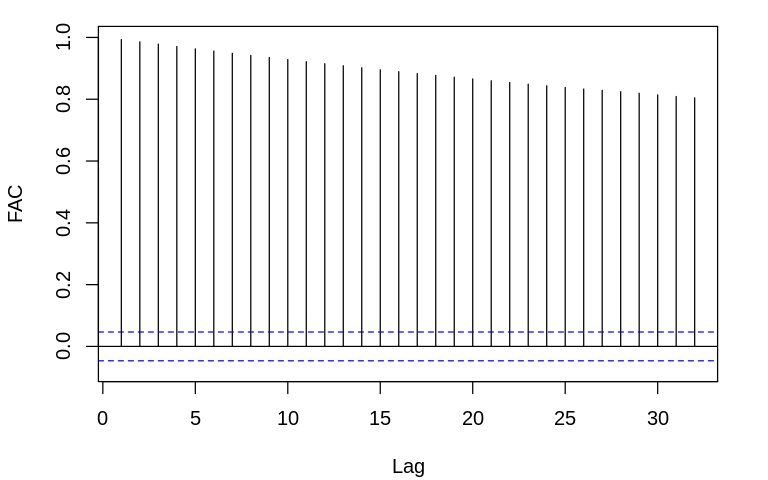
\includegraphics[width=.8\textwidth]{../images/SP500_FAC.png}
        \end{center}
    \end{block}
    \begin{itemize}
        \item Necessita de uma diferenciação
    \end{itemize}
\end{frame}

\begin{frame}{Análise da série}
    \begin{block}{Primeira diferenciação}
        \begin{columns}
            \begin{column}{.5\textwidth}
                \begin{center}
                    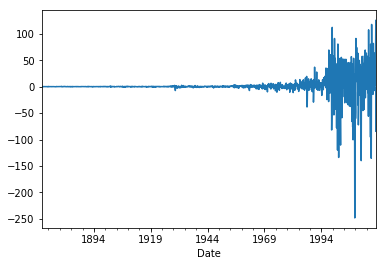
\includegraphics[width=.9\textwidth]{../images/sp500diff.png}
                \end{center}
            \end{column}
            \begin{column}{.5\textwidth}
                \begin{block}{FAC da diferenciação}
                    \begin{center}
                        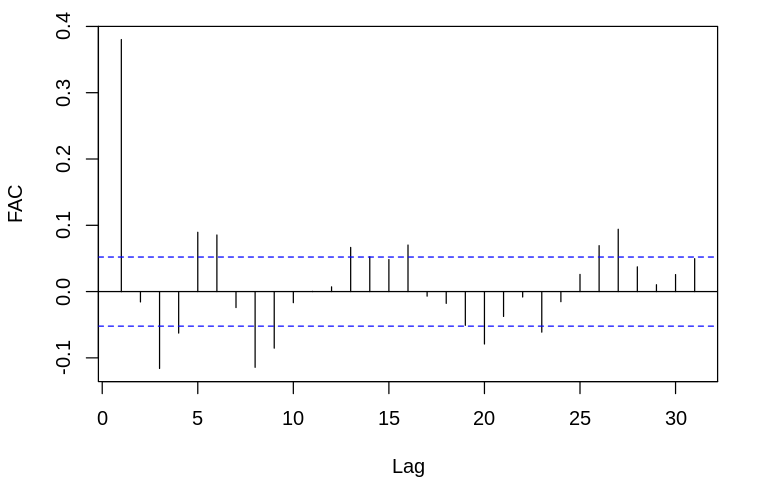
\includegraphics[width=.9\textwidth]{../images/SP500_diff_FAC.png}
                    \end{center}
                \end{block}
            \end{column}
        \end{columns}
    \end{block}
\end{frame}

\begin{frame}{Definição do modelo probabilístico}
    \begin{block}{FACP da série diferenciada}
        \begin{center}
            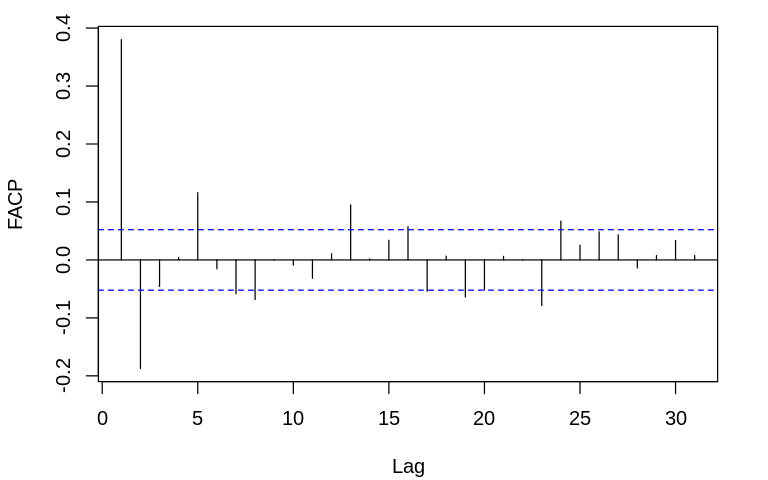
\includegraphics[width=.5\textwidth]{../images/SP500_diff_FACP.png}
        \end{center}
    \end{block}
    \begin{description}
        \item[AR\(p\)] \{1, 2 ou 5\}
        \item[MA\(q\)] \{1, 2 ou 7\}
    \end{description}
\end{frame}

\begin{frame}{Seleção do melhor modelo}
    Utilizando o \textbf{AIC}

    \begin{center}
        \begin{tabular}{l c c c}
                                & \multicolumn{3}{c}{$q$}           \\
            $p$                 & 1      & 2      & 7               \\
            \toprule
            1                   & -15953 & -15952 & -15979          \\
            2                   & -15965 & -15968 & -15989          \\
            5                   & -15984 & -15988 & \alert<2>{-16004} \\
        \end{tabular}
    \end{center}
\end{frame}

\begin{frame}{Validação dos resíduos}
    \begin{block}{FAC}
        \begin{center}
            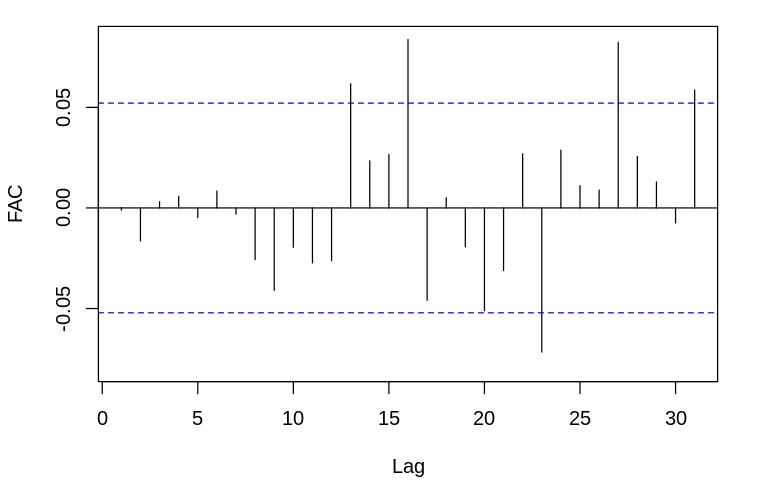
\includegraphics[width=.8\linewidth]{../images/residuals_FAC.png}
        \end{center}
    \end{block}
\end{frame}

\begin{frame}{Definição do Modelo utilizando redes neurais}
    \begin{block}{Busca em grade}
        \begin{center}
            \begin{tabular}{l l}
            \multicolumn{1}{c}{Parâmetro}        & \multicolumn{1}{c}{Possibilidades}  \\
                \toprule
                Número de camadas                & 1 \ldots 4                          \\
                Número de unidades por camada    & 1 \ldots 20                         \\
                $\lambda$ regularização          & 0.00001 \ldots 0.0001               \\
                Função de ativação               & $relu$, $sigmoid$                   \\
                Função de erro                   & MSE, MAE                            \\
                Iterações                        & 20 \ldots 500
            \end{tabular}
        \end{center}
    \end{block}
    \uncover<2->{
        \begin{block}{Modelo selecionado}
            Duas camadas, sendo a primeira com 13 neuronios e a de saída com um
            único neuronio.
            A função de ativação \textbf{relu} e a regularização 0,000001.
            Sendo \textbf{300} o números de iterações.
        \end{block}
    }
\end{frame}

\section{Resultados}

\begin{frame}{Resultados}
    \begin{block}{MSE dos modelos obtidos}
        \begin{center}
            \begin{tabular}{ll}
                \multicolumn{1}{c}{Modelo} & \multicolumn{1}{c}{MSE} \\
                \toprule
                MLP                        & 0,0002101               \\
                ARIMA                      & 0,0002088
            \end{tabular}
        \end{center}
    \end{block}
\end{frame}

\begin{frame}{Resultados}
    \begin{columns}
        \begin{column}{.5\textwidth}
            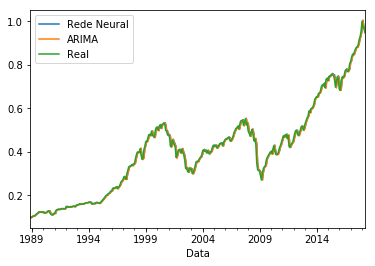
\includegraphics[width=\textwidth]{../images/sp500_prediction_compare.png}
        \end{column}
        \begin{column}{.5\textwidth}
            \begin{block}{Erros acumulados}
                \begin{center}
                    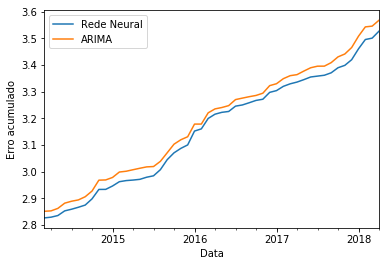
\includegraphics[width=.8\textwidth]{../images/sp500_cumsum.png}
                \end{center}
            \end{block}
        \end{column}
    \end{columns}
\end{frame}

\section{Conclusões}

% TODO faltas as conclusões :(

\section{Trabalhos futuros}

\begin{frame}{Trabalhos futuros}
    \begin{itemize}
        \item Modelis hibridos
        \item Redes neurais recorrents (LSTM)
        \item SARIMA e SARIMAX
    \end{itemize}
\end{frame}

\section{Referências}

\begin{frame}[allowframebreaks]{Referências}
    \nocite{box}
    \nocite{ehlers}
    \nocite{zhang}
    \bibliographystyle{apalike}
    \bibliography{../referencias}
\end{frame}

\end{document}
